% Falling single-arm pendulum: equations only, with the variable key on every page.
% Build: pdflatex falling_pendulum_math.tex (twice)
\documentclass[11pt]{article}
\usepackage[paperwidth=11in,paperheight=8.5in,left=0.6in,right=4.3in,top=0.55in,bottom=0.6in]{geometry}
\usepackage[T1]{fontenc}
\usepackage{lmodern}
\usepackage{amsmath,amssymb,mathtools,bm}
\usepackage{array,booktabs}
\usepackage{xcolor}
\usepackage{tikz}
\usetikzlibrary{arrows.meta,calc,patterns}
\usepackage{eso-pic}
\usepackage[most]{tcolorbox}
\usepackage{enumitem}
\usepackage[hidelinks]{hyperref}

\definecolor{accent}{HTML}{1F5FA8}
\definecolor{grav}{HTML}{C2410C}
\definecolor{keybg}{HTML}{F1F5FB}
\definecolor{muted}{HTML}{5B6878}

\newcommand{\sgn}{\operatorname{sgn}}
\newcommand{\Lag}{\mathcal{L}}
\newcommand{\Ray}{\mathcal{D}}
\setlength{\parindent}{0pt}
\setlength{\parskip}{4pt}
\allowdisplaybreaks

% ---------- boxed result with its own "where" list ----------
\newtcolorbox{result}[1][]{enhanced,colback=accent!4,colframe=accent,boxrule=0.8pt,arc=2pt,
  left=6pt,right=6pt,top=3pt,bottom=4pt,fonttitle=\bfseries\small,coltitle=white,#1}
\newcommand{\where}[1]{\par\vspace{-2pt}{\small\color{muted}\textit{where}}\par\vspace{-2pt}
  {\small\renewcommand{\arraystretch}{1.08}\begin{tabular}{@{}>{$}r<{$}@{\;\;}l@{}}#1\end{tabular}}}

% ---------- the variable key, printed down the right side of every page ----------
\newcommand{\kh}[1]{\multicolumn{3}{@{}l}{\rule{0pt}{10pt}\textbf{\color{accent}#1}}\\[0pt]}
\newcommand{\keypanel}{%
\begin{tcolorbox}[enhanced,width=3.7in,height=7.68in,colback=keybg,colframe=accent!60,boxrule=0.6pt,arc=3pt,
  left=5pt,right=5pt,top=4pt,bottom=4pt]
{\small\bfseries VARIABLE KEY}\hfill{\scriptsize\color{muted}SI units, angles in radians}\par\vspace{1pt}
\footnotesize\renewcommand{\arraystretch}{1.0}\setlength{\tabcolsep}{2.2pt}
\begin{tabular}{@{}>{$}l<{$}>{\raggedright\arraybackslash}p{2.08in}>{\raggedright\arraybackslash}p{0.74in}@{}}
\kh{Angle and time}
\theta & angle from straight up, clockwise $+$ & rad \\
 & \multicolumn{2}{@{}l}{\color{muted}$0$ = upright, $\pi/2$ = horizontal, $\pi$ = hanging}\\
\theta_0 & release angle (let go at rest) & rad \\
\dot\theta,\ \ddot\theta & angular velocity, acceleration & rad/s, rad/s$^2$ \\
t & time since release & s \\
\varphi & angle from hanging, $\theta-\pi$ & rad \\
\kh{Arm}
m & mass of everything that turns & kg \\
L & pivot to tip & m \\
l_c & pivot to centre of mass (CoM) & m \\
s & pivot to any chosen point & m \\
I & moment of inertia about the pivot & kg\,m$^2$ \\
I_{cm} & moment of inertia about the CoM & kg\,m$^2$ \\
g & gravitational acceleration & m/s$^2$ \\
\kh{Friction and torques}
b & viscous friction coefficient & N\,m\,s/rad \\
\tau_c & Coulomb (dry) friction torque & N\,m \\
\tau_s & static friction torque, $\ge\tau_c$ & N\,m \\
\tau_f & total friction torque on the arm & N\,m \\
\tau & motor torque (0 while falling) & N\,m \\
\sgn & sign: $+1$, $0$ or $-1$ & -- \\
\kh{Derived constants}
k & $m g l_c$, gravity stiffness & N\,m/rad \\
\omega_n & $\sqrt{k/I}$, natural frequency & rad/s \\
T_n & $2\pi/\omega_n$, small hanging-swing period & s \\
\zeta & $b/(2\sqrt{Ik})$, damping ratio & -- \\
\omega_d & $\omega_n\sqrt{1-\zeta^2}$, damped frequency & rad/s \\
\theta_c & $\tau_c/k$, Coulomb offset & rad \\
r_1,\ r_2 & growth, decay rate near upright & 1/s \\
\kappa,\ \beta & elliptic modulus $\cos\frac{\theta_0}{2}$; elliptic angle & --, rad \\
F,\ K,\ \mathrm{sn} & elliptic integrals, Jacobi sine & -- \\
A_n & amplitude of swing $n$ & rad \\
\kh{Motion and forces}
x,\ y & position of a point (origin at pivot) & m \\
\dot x,\dot y;\ \ddot x,\ddot y & velocity; acceleration of that point & m/s; m/s$^2$ \\
v,\ a_t,\ a_n & speed; tangential, centripetal accel. & m/s; m/s$^2$ \\
R_x,\ R_y & force of the pivot on the arm & N \\
\kh{Energy and numerics}
T,\ V & kinetic, potential energy & J \\
\Lag & Lagrangian $T-V$ & J \\
\Ray & Rayleigh dissipation $\tfrac12 b\dot\theta^2$ & W \\
Q_c & Coulomb generalized torque & N\,m \\
E & total energy (0 = hanging at rest) & J \\
\bm z,\ h & state $[\theta,\dot\theta]$; RK4 time step & --; s \\
\end{tabular}
\end{tcolorbox}}
\AddToShipoutPictureBG{\AtPageLowerLeft{\put(\LenToUnit{6.92in},\LenToUnit{0.4in}){\parbox[b]{3.7in}{\keypanel}}}}

\begin{document}

%=====================================================================
{\LARGE\bfseries Falling Single-Arm Pendulum}\par\vspace{2pt}
{\large Equations of motion and kinematics: fixed pivot, released from rest at any angle, with moment of inertia, viscous and Coulomb friction}\par\vspace{4pt}
{\small\color{muted}ENGT 480 Pendulum team (Ryan Barney) \quad 2026-11-20 \quad Every symbol is defined in the key on the right of every page. Formulas use SI units and radians.}

\vspace{6pt}
\begin{minipage}[t]{0.47\linewidth}
\vspace{0pt}
\centering
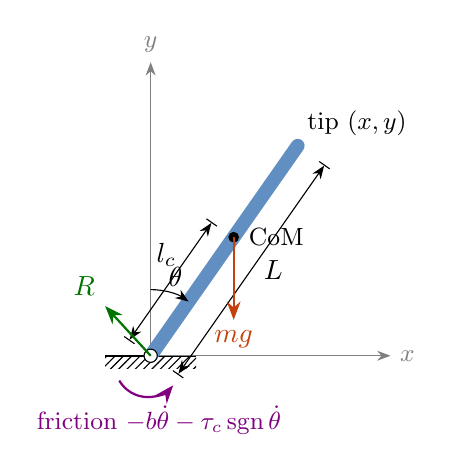
\begin{tikzpicture}[scale=1.05,>=Stealth]
  \fill[pattern=north east lines] (-0.55,0) rectangle (0.55,-0.16);
  \draw[thick] (-0.55,0)--(0.55,0);
  \draw[->,gray] (0,0)--(0,3.55) node[above]{\small $y$};
  \draw[->,gray] (0,0)--(2.9,0) node[right]{\small $x$};
  \def\th{35}
  \coordinate (O) at (0,0);
  \coordinate (C) at ({1.75*sin(\th)},{1.75*cos(\th)});
  \coordinate (T) at ({3.1*sin(\th)},{3.1*cos(\th)});
  \draw[line width=5pt,accent!70,line cap=round] (O)--(T);
  \fill[white] (O) circle (0.08); \draw (O) circle (0.08);
  \fill (C) circle (0.065);
  \node[right=2pt,font=\small] at (C) {CoM};
  \node[above right,font=\small] at (T) {tip $(x,y)$};
  \draw[->] (0,0.8) arc (90:{90-\th}:0.8);
  \node at ({1.0*sin(\th/2)},{1.0*cos(\th/2)}) {$\theta$};
  \draw[|<->|,thin] ($(O)+({-0.32*cos(\th)},{0.32*sin(\th)})$) -- ($(C)+({-0.32*cos(\th)},{0.32*sin(\th)})$) node[pos=0.72,left=1pt]{$l_c$};
  \draw[|<->|,thin] ($(O)+({0.4*cos(\th)},{-0.4*sin(\th)})$) -- ($(T)+({0.4*cos(\th)},{-0.4*sin(\th)})$) node[midway,right=1pt]{$L$};
  \draw[->,thick,grav] (C)--++(0,-1.0) node[below]{$mg$};
  \draw[->,thick,green!45!black] (O)--++(-0.55,0.6) node[above left]{$R$};
  \draw[->,thick,violet] (-0.38,-0.3) arc (210:320:0.4);
  \node[violet,font=\small] at (0.1,-0.78) {friction $-b\dot\theta-\tau_c\sgn\dot\theta$};
\end{tikzpicture}
\end{minipage}\hfill
\begin{minipage}[t]{0.5\linewidth}
\vspace{4pt}
\textbf{Sign convention}
\begin{itemize}[leftmargin=12pt,itemsep=1pt,topsep=2pt]
\item $\theta$ is measured from straight \textbf{up}, clockwise positive (tip moves to $+x$).
\item $\theta=0$ upright, $\theta=\pi/2$ horizontal, $\theta=\pi$ hanging. $\theta$ is not wrapped: after the bottom it keeps growing ($3\pi/2$ is horizontal on the other side).
\item Pivot at the origin, $y$ up, pivot fixed.
\item Released at rest: $\theta(0)=\theta_0$, $\dot\theta(0)=0$.
\end{itemize}
\textbf{Assumptions:} rigid arm, planar motion, air drag lumped into $b$, no motor ($\tau=0$) unless stated.
\end{minipage}

\vspace{8pt}
\textbf{Contents.} 1 All equations on one page \textperiodcentered{} 2 Moment of inertia \textperiodcentered{} 3 Forward kinematics \textperiodcentered{} 4 Inverse kinematics \textperiodcentered{} 5 Equation of motion (Lagrange) \textperiodcentered{} 6 Friction model \textperiodcentered{} 7 State-space form \textperiodcentered{} 8 Energy \textperiodcentered{} 9 Exact solution without friction \textperiodcentered{} 10 Small angles near upright \textperiodcentered{} 11 Small swings near hanging \textperiodcentered{} 12 Pivot force \textperiodcentered{} 13 Inverse dynamics \textperiodcentered{} 14 Numerical solution \textperiodcentered{} 15 Numbers for V2 arm 1

\newpage
%=====================================================================
\section*{1\quad All equations on one page}
\renewcommand{\arraystretch}{1.55}
\begin{tabular}{@{}>{\raggedright\arraybackslash}p{1.35in}l@{}}
\textbf{Inertia} & $I = I_{cm} + m l_c^2$ \qquad (uniform rod: $I=\tfrac13 mL^2$, $l_c=\tfrac L2$)\\
\textbf{Equation of motion} & $I\ddot\theta = m g l_c\sin\theta - b\dot\theta - \tau_c\sgn\dot\theta$, \quad $\theta(0)=\theta_0,\ \dot\theta(0)=0$\\
\textbf{Does it fall?} & yes if $m g l_c|\sin\theta_0| > \tau_s$\\
\textbf{Point position} & $x = s\sin\theta,\quad y = s\cos\theta$ \qquad (tip $s=L$, CoM $s=l_c$)\\
\textbf{Point velocity} & $\dot x = s\dot\theta\cos\theta,\quad \dot y = -s\dot\theta\sin\theta$\\
\textbf{Point acceleration} & $\ddot x = s(\ddot\theta\cos\theta-\dot\theta^2\sin\theta),\quad \ddot y = -s(\ddot\theta\sin\theta+\dot\theta^2\cos\theta)$\\
\textbf{Inverse kinematics} & $\theta=\operatorname{atan2}(x,y),\quad \dot\theta=\dfrac{y\dot x-x\dot y}{x^2+y^2},\quad \ddot\theta=\dfrac{y\ddot x-x\ddot y}{x^2+y^2}$\\
\textbf{Energy} & $E=\tfrac12 I\dot\theta^2+m g l_c(1+\cos\theta),\qquad \dot E = -b\dot\theta^2-\tau_c|\dot\theta|$\\
\textbf{Speed, no friction} & $\dot\theta=\sqrt{2\omega_n^2(\cos\theta_0-\cos\theta)}$\\
\textbf{$\theta(t)$, no friction} & $\theta(t)=\pi-2\arcsin\!\big[\kappa\,\mathrm{sn}(K(\kappa)-\omega_n t,\ \kappa)\big],\quad \kappa=\cos\tfrac{\theta_0}{2}$\\
\textbf{Time to angle, no friction} & $t(\theta)=\dfrac{K(\kappa)-F(\beta,\kappa)}{\omega_n},\quad \sin\beta=\dfrac{\sin\frac{\pi-\theta}{2}}{\kappa},\quad t_{bottom}=\dfrac{K(\kappa)}{\omega_n}$\\
\textbf{Near upright (small $\theta$)} & $\theta(t)=\theta_c+(\theta_0-\theta_c)\dfrac{r_1e^{r_2t}-r_2e^{r_1t}}{r_1-r_2},\quad \theta_c=\dfrac{\tau_c}{k}$\\
 & $r_{1,2}=-\dfrac{b}{2I}\pm\sqrt{\Big(\dfrac{b}{2I}\Big)^2+\dfrac{k}{I}}$\\
\textbf{Near hanging (small $\varphi$)} & $\varphi(t)=\varphi_0e^{-\zeta\omega_nt}\Big(\cos\omega_dt+\dfrac{\zeta}{\sqrt{1-\zeta^2}}\sin\omega_dt\Big)$ \quad (viscous only)\\
\textbf{Pivot force} & $R_x=m l_c(\ddot\theta\cos\theta-\dot\theta^2\sin\theta),\quad R_y=m g-m l_c(\ddot\theta\sin\theta+\dot\theta^2\cos\theta)$\\
\textbf{Motor torque to follow $\theta(t)$} & $\tau=I\ddot\theta-m g l_c\sin\theta+b\dot\theta+\tau_c\sgn\dot\theta$\\
\textbf{With friction, any angle} & no closed form: solve numerically (Section 14)\\
\end{tabular}
\renewcommand{\arraystretch}{1}

\newpage
%=====================================================================
\section*{2\quad Moment of inertia}
Every bit of mass $dm$ at distance $r$ from the pivot adds $r^2\,dm$. Measured about the CoM and moved to the pivot with the parallel-axis theorem:
\begin{result}
\begin{equation}
I = I_{cm} + m\,l_c^2
\end{equation}
\where{I & moment of inertia about the pivot (kg\,m$^2$)\\ I_{cm} & moment of inertia about the centre of mass (kg\,m$^2$)\\ m & arm mass (kg)\\ l_c & pivot to centre of mass (m)}
\end{result}
Uniform thin rod of length $L$ pivoted at one end:
\begin{equation}
l_c=\frac{L}{2},\qquad I_{cm}=\frac{mL^2}{12},\qquad I=\frac{mL^2}{12}+m\Big(\frac{L}{2}\Big)^2=\frac{mL^2}{3}.
\end{equation}
For a real arm (hub, magnet, battery, holes) use the CAD value or measure it from the small hanging-swing period: $I = m g l_c\,(T_n/2\pi)^2$ (from Section 11).

%=====================================================================
\section*{3\quad Forward kinematics: where every point is}
A point at distance $s$ from the pivot (tip: $s=L$; CoM: $s=l_c$). Once $\theta(t)$ is known, these give the point at any time.
\begin{result}
\begin{align}
x &= s\sin\theta, & y &= s\cos\theta \label{eq:pos}\\
\dot x &= s\,\dot\theta\cos\theta, & \dot y &= -s\,\dot\theta\sin\theta \label{eq:vel}\\
\ddot x &= s\big(\ddot\theta\cos\theta-\dot\theta^2\sin\theta\big), & \ddot y &= -s\big(\ddot\theta\sin\theta+\dot\theta^2\cos\theta\big) \label{eq:acc}
\end{align}
\where{x,\ y & position of the point, pivot at the origin, $y$ up (m)\\ s & pivot to the point (m)\\ \theta,\ \dot\theta,\ \ddot\theta & angle (rad), angular velocity (rad/s), angular acceleration (rad/s$^2$)}
\end{result}
Each line is the time derivative of the one above it (chain rule: $\tfrac{d}{dt}\sin\theta=\dot\theta\cos\theta$, $\tfrac{d}{dt}\cos\theta=-\dot\theta\sin\theta$).
Split along and across the arm:
\begin{equation}
v = s|\dot\theta|,\qquad a_t = s\ddot\theta\ \ \text{(along the motion)},\qquad a_n = s\dot\theta^2\ \ \text{(toward the pivot)}.
\end{equation}

%=====================================================================
\section*{4\quad Inverse kinematics: from a point back to the angle}
Given a measured point (camera, tracker) and its derivatives:
\begin{result}
\begin{gather}
\theta = \operatorname{atan2}(x,\ y),\qquad s=\sqrt{x^2+y^2} \label{eq:ik}\\[2pt]
\dot\theta = \frac{y\,\dot x - x\,\dot y}{x^2+y^2},\qquad
\ddot\theta = \frac{y\,\ddot x - x\,\ddot y}{x^2+y^2} \label{eq:ikd}
\end{gather}
\where{x,\ y & measured position of the point (m)\\ \dot x,\dot y;\ \ddot x,\ddot y & its velocity (m/s); acceleration (m/s$^2$)\\ \theta & arm angle from straight up (rad)}
\end{result}
\textbf{Argument order:} $\operatorname{atan2}(x,y)$, not $(y,x)$, because $\theta$ is measured from the $+y$ axis.

\textbf{Proof of \eqref{eq:ikd}.} Substitute \eqref{eq:pos} and \eqref{eq:vel}:
\begin{equation*}
y\dot x - x\dot y = (s\cos\theta)(s\dot\theta\cos\theta)-(s\sin\theta)(-s\dot\theta\sin\theta)=s^2\dot\theta(\cos^2\theta+\sin^2\theta)=s^2\dot\theta .
\end{equation*}
With \eqref{eq:acc} the $\dot\theta^2$ terms cancel the same way: $y\ddot x-x\ddot y=s^2\ddot\theta$. Divide by $s^2=x^2+y^2$.

%=====================================================================
\section*{5\quad Equation of motion by Lagrange}
\textbf{Step 1: coordinate.} One degree of freedom, the angle $\theta$.

\textbf{Step 2: kinetic energy.} The arm turns about a fixed point, so all of its kinetic energy is rotation about the pivot:
\begin{equation}
T=\tfrac12 I\dot\theta^2 \qquad\Big(=\tfrac12 m (l_c\dot\theta)^2+\tfrac12 I_{cm}\dot\theta^2,\ \text{same thing by Section 2}\Big).
\end{equation}

\textbf{Step 3: potential energy.} The CoM is $l_c\cos\theta$ above the pivot:
\begin{equation}
V = m g l_c\cos\theta .
\end{equation}

\textbf{Step 4: Lagrangian.}
\begin{equation}
\Lag = T - V = \tfrac12 I\dot\theta^2 - m g l_c\cos\theta .
\end{equation}

\textbf{Step 5: friction.} Viscous friction enters through the Rayleigh dissipation function, Coulomb friction as a generalized torque:
\begin{equation}
\Ray=\tfrac12 b\dot\theta^2,\qquad Q_c=-\tau_c\sgn\dot\theta .
\end{equation}

\textbf{Step 6: Lagrange's equation with dissipation.}
\begin{equation}
\frac{d}{dt}\!\left(\frac{\partial\Lag}{\partial\dot\theta}\right)-\frac{\partial\Lag}{\partial\theta}+\frac{\partial\Ray}{\partial\dot\theta}=Q_c+\tau .
\end{equation}

\textbf{Step 7: the derivatives.}
\begin{equation}
\frac{\partial\Lag}{\partial\dot\theta}=I\dot\theta\ \Rightarrow\ \frac{d}{dt}\Big(\frac{\partial\Lag}{\partial\dot\theta}\Big)=I\ddot\theta,\qquad
\frac{\partial\Lag}{\partial\theta}=m g l_c\sin\theta,\qquad
\frac{\partial\Ray}{\partial\dot\theta}=b\dot\theta .
\end{equation}

\textbf{Step 8: substitute} (falling freely, $\tau=0$):
\begin{result}[title={Equation of motion}]
\begin{equation}
I\ddot\theta = m g l_c\sin\theta - b\dot\theta - \tau_c\sgn\dot\theta,\qquad \theta(0)=\theta_0,\quad \dot\theta(0)=0 \label{eq:eom}
\end{equation}
\where{I & moment of inertia about the pivot (kg\,m$^2$)\\ m g l_c\sin\theta & gravity torque, pushes the arm away from upright (N\,m)\\ b\dot\theta & viscous friction torque, $b$ in N\,m\,s/rad\\ \tau_c\sgn\dot\theta & Coulomb friction torque, always against the motion (N\,m)\\ \theta_0 & release angle (rad), arm let go at rest}
\end{result}
Divided by $I$, with $\omega_n^2=m g l_c/I$:
\begin{equation}
\ddot\theta=\omega_n^2\sin\theta-\frac{b}{I}\dot\theta-\frac{\tau_c}{I}\sgn\dot\theta . \label{eq:eomI}
\end{equation}
\textbf{Newton check.} Torques about the pivot (the pivot force $R$ has no moment arm): gravity $+m g l_c\sin\theta$, friction $-b\dot\theta-\tau_c\sgn\dot\theta$; $\sum\tau = I\ddot\theta$ gives \eqref{eq:eom} again.

%=====================================================================
\section*{6\quad Friction model}
\begin{equation}
\sgn\dot\theta=\begin{cases}+1 & \dot\theta>0\\ \ \ 0 & \dot\theta=0\\ -1 & \dot\theta<0\end{cases}
\end{equation}
While the arm is stopped, dry friction supplies whatever torque keeps it stopped, up to $\tau_s$. So the full friction torque on the arm is
\begin{result}
\begin{equation}
\tau_f=\begin{cases}
-b\dot\theta-\tau_c\sgn\dot\theta & \dot\theta\neq0 \ \text{(sliding)}\\[2pt]
-m g l_c\sin\theta & \dot\theta=0 \text{ and } m g l_c|\sin\theta|\le\tau_s\ \text{(stuck)}\\[2pt]
-\tau_c\sgn(\sin\theta) & \dot\theta=0 \text{ and } m g l_c|\sin\theta|>\tau_s\ \text{(breaking away)}
\end{cases}
\end{equation}
\where{\tau_f & total friction torque on the arm (N\,m); the motion is $I\ddot\theta=m g l_c\sin\theta+\tau_f$\\ \tau_s & static friction torque (N\,m), $\tau_s\ge\tau_c$; use $\tau_s=\tau_c$ if unknown}
\end{result}
\textbf{Does it fall at all?} Only if gravity beats static friction at the release angle:
\begin{equation}
m g l_c|\sin\theta_0|>\tau_s\quad\Longleftrightarrow\quad |\theta_0|>\arcsin\frac{\tau_s}{m g l_c}.
\end{equation}

%=====================================================================
\section*{7\quad State-space form}
Two first-order equations, the form a computer integrates:
\begin{result}
\begin{equation}
\bm z=\begin{bmatrix}\theta\\ \dot\theta\end{bmatrix},\qquad
\dot{\bm z}=\bm f(\bm z)=\begin{bmatrix}\dot\theta\\[2pt] \dfrac{1}{I}\big(m g l_c\sin\theta+\tau_f\big)\end{bmatrix},\qquad
\bm z(0)=\begin{bmatrix}\theta_0\\ 0\end{bmatrix} \label{eq:ss}
\end{equation}
\where{\bm z & state vector (rad, rad/s)\\ \tau_f & friction torque from Section 6 (N\,m)}
\end{result}
Only three ratios set $\theta(t)$: $\omega_n^2=m g l_c/I$, $b/I$ and $\tau_c/I$. Scaling every mass and inertia by the same factor changes nothing.

%=====================================================================
\section*{8\quad Energy}
\begin{result}
\begin{equation}
E=\tfrac12 I\dot\theta^2+m g l_c(1+\cos\theta) \label{eq:E}
\end{equation}
\where{E & total mechanical energy (J), zero when hanging at rest ($\theta=\pi$)\\ \tfrac12 I\dot\theta^2 & kinetic energy\\ m g l_c(1+\cos\theta) & potential energy above the hanging position}
\end{result}
Multiply \eqref{eq:eom} by $\dot\theta$; the left side becomes $\tfrac{d}{dt}(\tfrac12 I\dot\theta^2)$ and $m g l_c\sin\theta\,\dot\theta=-\tfrac{d}{dt}\big(m g l_c\cos\theta\big)$, so
\begin{equation}
\frac{dE}{dt}=-b\dot\theta^2-\tau_c|\dot\theta|\ \le 0 .
\end{equation}
Friction only removes energy. With no friction $E$ is constant, which is what makes Section 9 solvable.

%=====================================================================
\section*{9\quad Exact solution without friction ($b=\tau_c=0$)}
\textbf{Speed at any angle.} $E$ at release equals $E$ at angle $\theta$:
$\ m g l_c(1+\cos\theta_0)=\tfrac12 I\dot\theta^2+m g l_c(1+\cos\theta)$, so
\begin{result}
\begin{equation}
\dot\theta(\theta)=\sqrt{2\omega_n^2\big(\cos\theta_0-\cos\theta\big)},\qquad
\dot\theta_{bottom}=\omega_n\sqrt{2(1+\cos\theta_0)}\ \le\ 2\omega_n \label{eq:speed}
\end{equation}
\where{\omega_n & $\sqrt{m g l_c/I}$ (rad/s)\\ \dot\theta_{bottom} & angular speed passing the bottom, $\theta=\pi$ (rad/s)}
\end{result}

\textbf{Time to reach any angle.} Separate variables, $dt=d\theta/\dot\theta$:
\begin{equation}
t(\theta)=\int_{\theta_0}^{\theta}\frac{d\vartheta}{\sqrt{2\omega_n^2(\cos\theta_0-\cos\vartheta)}} . \label{eq:tint}
\end{equation}
With the substitution $\sin\frac{\pi-\vartheta}{2}=\kappa\sin\phi$ this becomes a standard elliptic integral:
\begin{result}
\begin{gather}
t(\theta)=\frac{K(\kappa)-F(\beta,\kappa)}{\omega_n},\qquad
t_{bottom}=\frac{K(\kappa)}{\omega_n} \label{eq:ell}\\[2pt]
\kappa=\cos\frac{\theta_0}{2},\qquad
\sin\beta=\frac{\sin\frac{\pi-\theta}{2}}{\kappa} \nonumber
\end{gather}
\where{F(\beta,\kappa) & $\displaystyle\int_0^{\beta}\frac{d\phi}{\sqrt{1-\kappa^2\sin^2\phi}}$, incomplete elliptic integral of the first kind\\ K(\kappa) & $F(\pi/2,\kappa)$, complete elliptic integral\\ t(\theta) & time from release to angle $\theta$, valid for $\theta_0\le\theta\le\pi$ (s)}
\end{result}

\textbf{Angle at any time.} Inverting \eqref{eq:ell} with the Jacobi sine $\mathrm{sn}$ (the inverse of $F$: $\mathrm{sn}(u,\kappa)=\sin\beta$ when $u=F(\beta,\kappa)$):
\begin{result}
\begin{equation}
\theta(t)=\pi-2\arcsin\!\Big[\kappa\,\mathrm{sn}\big(K(\kappa)-\omega_n t,\ \kappa\big)\Big] \label{eq:sn}
\end{equation}
\where{\mathrm{sn}(u,\kappa) & Jacobi elliptic sine (in SciPy: \texttt{scipy.special.ellipj(u, kappa**2)[0]})\\ & valid for all $t$: gives $\theta_0$ at $t=0$, $\pi$ at $t_{bottom}$, then swings to $2\pi-\theta_0$ and back}
\end{result}
Check: $t=0$ gives $\mathrm{sn}(K)=1$ and $\theta=\pi-2\arcsin(\cos\frac{\theta_0}{2})=\theta_0$. As $\theta_0\to0$, $\kappa\to1$ and $K\to\infty$: an arm balanced exactly upright never falls.

%=====================================================================
\section*{10\quad Small angles near upright (falling phase)}
\textbf{Linearize.} For small $\theta$, $\sin\theta\approx\theta$. Falling from $\theta_0>0$ the arm moves with $\dot\theta>0$, so $\sgn\dot\theta=+1$ and \eqref{eq:eom} becomes linear:
\begin{equation}
I\ddot\theta+b\dot\theta-k\theta=-\tau_c,\qquad k=m g l_c .
\end{equation}
\textbf{Shift out the constant.} Let $u=\theta-\theta_c$ with $\theta_c=\tau_c/k$:
\begin{equation}
I\ddot u+b\dot u-k u=0 .
\end{equation}
\textbf{Characteristic equation.} Try $u=e^{rt}$: $I r^2+b r-k=0$, so
\begin{equation}
r_{1,2}=-\frac{b}{2I}\pm\sqrt{\Big(\frac{b}{2I}\Big)^2+\frac{k}{I}},\qquad r_1>0>r_2 .
\end{equation}
\textbf{Initial conditions.} $u=Ae^{r_1t}+Be^{r_2t}$ with $u(0)=\theta_0-\theta_c$ and $\dot u(0)=0$ gives $A=\dfrac{-r_2(\theta_0-\theta_c)}{r_1-r_2}$, $B=\dfrac{r_1(\theta_0-\theta_c)}{r_1-r_2}$.
\begin{result}[title={Small-angle fall from upright}]
\begin{gather}
\theta(t)=\theta_c+(\theta_0-\theta_c)\,\frac{r_1e^{r_2t}-r_2e^{r_1t}}{r_1-r_2} \label{eq:lin}\\[2pt]
\dot\theta(t)=(\theta_0-\theta_c)\,\frac{r_1r_2\big(e^{r_2t}-e^{r_1t}\big)}{r_1-r_2}
\end{gather}
\where{r_1 & growth rate (1/s): the angle grows $e$-fold every $1/r_1$\\ r_2 & decay rate (1/s), negative\\ \theta_c & $\tau_c/(m g l_c)$, Coulomb offset (rad); needs $\theta_0>\theta_c$ to fall\\ & valid while $\theta$ is small: within 1\,\% to about $40^\circ$, 5\,\% to about $85^\circ$ (V2 arm 1)}
\end{result}
\textbf{No friction:} $r_{1,2}=\pm\omega_n$ and \eqref{eq:lin} becomes $\theta(t)=\theta_0\cosh(\omega_n t)$.

\textbf{Time to reach $\theta$} (once the $e^{r_2t}$ term has died out, $t\gtrsim1/r_1$):
\begin{equation}
t(\theta)\approx\frac{1}{r_1}\ln\!\left[\frac{(\theta-\theta_c)(r_1-r_2)}{-r_2\,(\theta_0-\theta_c)}\right]
\qquad\Big(\text{no friction: } t\approx\frac{1}{\omega_n}\ln\frac{2\theta}{\theta_0}\Big).
\end{equation}
Halving $\theta_0$ adds $\ln 2/r_1$ to every fall time. For $\theta_0<0$ the motion is the mirror image: use $|\theta_0|$ and flip the sign of the result.

%=====================================================================
\section*{11\quad Small swings near hanging}
Let $\varphi=\theta-\pi$. Then $\sin\theta=-\sin\varphi\approx-\varphi$ and \eqref{eq:eom} becomes
\begin{equation}
I\ddot\varphi+b\dot\varphi+k\varphi=-\tau_c\sgn\dot\varphi .
\end{equation}
\textbf{Viscous friction only,} released at rest from $\varphi_0$ (a free-swing test):
\begin{result}
\begin{equation}
\varphi(t)=\varphi_0\,e^{-\zeta\omega_nt}\Big(\cos\omega_dt+\frac{\zeta}{\sqrt{1-\zeta^2}}\sin\omega_dt\Big),\qquad
\frac{A_{n+1}}{A_n}=e^{-2\pi\zeta/\sqrt{1-\zeta^2}}
\end{equation}
\where{\varphi_0 & release angle from hanging (rad)\\ \zeta & damping ratio $b/(2\sqrt{I m g l_c})$\\ \omega_d & damped frequency $\omega_n\sqrt{1-\zeta^2}$ (rad/s)\\ A_n & amplitude of swing $n$; the ratio is per full period}
\end{result}
\textbf{Coulomb friction only:} the amplitude drops by a fixed amount every half swing, and the arm sticks once the amplitude is below $\tau_s/k$:
\begin{equation}
A_{n+\frac12}=A_n-\frac{2\tau_c}{k}.
\end{equation}
Exponential decay means viscous friction, straight-line decay means Coulomb friction; this is how $b$ and $\tau_c$ are measured. Large swings take longer than $T_n$: the period is $4K\!\big(\sin\frac{\varphi_0}{2}\big)/\omega_n$.

%=====================================================================
\section*{12\quad Pivot force}
Newton's second law for the centre of mass, with gravity $(0,-mg)$ and the CoM acceleration from \eqref{eq:acc} at $s=l_c$:
\begin{result}
\begin{align}
R_x &= m l_c\big(\ddot\theta\cos\theta-\dot\theta^2\sin\theta\big)\\
R_y &= m g - m l_c\big(\ddot\theta\sin\theta+\dot\theta^2\cos\theta\big)
\end{align}
\where{R_x,\ R_y & force the pivot puts on the arm, $x$ right, $y$ up (N); the bearing feels the opposite}
\end{result}
Passing the bottom ($\theta=\pi$, $\ddot\theta\approx0$) after a frictionless fall, with \eqref{eq:speed}:
\begin{equation}
R_y\approx m g+m l_c\dot\theta_{bottom}^2=m g\left[1+\frac{2 m l_c^2(1+\cos\theta_0)}{I}\right].
\end{equation}

%=====================================================================
\section*{13\quad Inverse dynamics: torque to follow a chosen motion}
Solve the equation of motion with a motor torque $\tau$ for $\tau$:
\begin{result}
\begin{equation}
\tau=I\ddot\theta-m g l_c\sin\theta+b\dot\theta+\tau_c\sgn\dot\theta
\end{equation}
\where{\tau & motor torque on the arm (N\,m) needed for a desired $\theta(t)$, $\dot\theta(t)$, $\ddot\theta(t)$}
\end{result}
Holding the arm still at $\theta$: $\tau=-m g l_c\sin\theta$, give or take $\tau_s$.

%=====================================================================
\section*{14\quad Numerical solution (any angle, with friction)}
With friction there is no closed form for $\theta(t)$: the equation is nonlinear ($\sin\theta$), friction breaks energy conservation, and Coulomb friction is discontinuous. Integrate \eqref{eq:ss} with 4th-order Runge--Kutta, step $h$:
\begin{result}
\begin{align}
\bm k_1&=\bm f(\bm z_n), & \bm k_2&=\bm f\big(\bm z_n+\tfrac h2\bm k_1\big), \nonumber\\
\bm k_3&=\bm f\big(\bm z_n+\tfrac h2\bm k_2\big), & \bm k_4&=\bm f\big(\bm z_n+h\bm k_3\big), \\
\bm z_{n+1}&=\bm z_n+\tfrac h6\big(\bm k_1+2\bm k_2+2\bm k_3+\bm k_4\big) \nonumber
\end{align}
\where{\bm z_n & state $[\theta,\dot\theta]$ at time $t_n=nh$\\ h & time step (s); $h=0.2$\,ms keeps the error under $0.001^\circ$ for this arm}
\end{result}
Then \eqref{eq:pos}--\eqref{eq:acc} give every point on the arm at every step. Checked against the exact formula \eqref{eq:ell}: fall times agree to better than $10^{-6}$\,s. Python version: \texttt{falling\_pendulum.py} in the same folder.

%=====================================================================
\section*{15\quad Numbers for V2 arm 1 (arm alone, cart locked)}
\begin{center}\renewcommand{\arraystretch}{1.1}
\begin{tabular}{cccc}
\toprule
$m$ & $L$ & $l_c$ & $g$\\
0.0981 kg & 0.200 m & 0.1478 m & 9.81 m/s$^2$\\
\midrule
$I$ & $I_{cm}$ & $b$ & $\tau_c$\\
$2.484\times10^{-3}$ kg\,m$^2$ & $3.40\times10^{-4}$ kg\,m$^2$ & $1.63\times10^{-4}$ N\,m\,s/rad & 0 (not measured)\\
\bottomrule
\end{tabular}\end{center}
\textbf{Sources: }$m$, $l_c$, $I$, $I_{cm}$ from the team's STL model with measured weights (PUC \texttt{params.md}, 2026-10-29); it predicts $T_n=0.830$\,s against 0.84--0.89\,s measured on the rig. $b=B_1J_1=0.0182\times8.96\times10^{-3}$ from the 2026-11-04 rig fit, which had arm 2 attached, so it is an estimate for the arm alone. $\tau_c$ has not been measured.

\textbf{Substituted:}
\begin{align*}
k&=m g l_c=0.0981\times9.81\times0.1478=0.1422\ \text{N\,m/rad}\\
\omega_n&=\sqrt{k/I}=\sqrt{0.1422/0.002484}=7.567\ \text{rad/s},\qquad T_n=2\pi/\omega_n=0.830\ \text{s}\\
\zeta&=\frac{b}{2\sqrt{Ik}}=\frac{1.63\times10^{-4}}{2\sqrt{0.002484\times0.1422}}=0.0043\\
r_{1,2}&=-0.0328\pm\sqrt{0.0328^2+57.26}=+7.534,\ -7.600\ \text{1/s}
\end{align*}
\textbf{Released from $\theta_0=10^\circ$:}
\begin{center}
\renewcommand{\arraystretch}{1.15}
\begin{tabular}{lrr}
\toprule
 & with rig $b$ & no friction, exact \eqref{eq:ell}\\
\midrule
time to horizontal, $\theta=90^\circ$ & 0.3905 s & 0.3893 s\\
time to bottom, $\theta=180^\circ$ & 0.5083 s & 0.5064 s\\
speed at bottom, $\dot\theta_{bottom}$ & 856 $^\circ$/s & 864 $^\circ$/s\\
tip speed at bottom, $L\dot\theta_{bottom}$ & 2.99 m/s & 3.02 m/s\\
pivot force at bottom, $|R|$ & 4.2 N ($4.4\,mg$) & 4.3 N\\
\bottomrule
\end{tabular}
\end{center}
Fall time to the bottom for other release angles (rig $b$): $1^\circ$: 0.813 s, $5^\circ$: 0.600 s, $10^\circ$: 0.508 s, $30^\circ$: 0.367 s, $60^\circ$: 0.286 s.

\end{document}
